\documentclass{beamer}

\usetheme{CambridgeUS}

\usepackage[utf8]{inputenc}
\usepackage[T1]{fontenc}

\usepackage{CJKutf8}
\usepackage{datetime}
\usepackage{amsmath}
\usepackage{amssymb}
\usepackage{mathtools}
\usepackage{subcaption}
\usepackage{minted}
\usepackage{xcolor}
\usepackage{ulem}
\usepackage{hyperref}
\usepackage{graphicx}
\usepackage{cite}
\usepackage{multirow}
\usepackage{makecell}
\usepackage{url}
\usepackage{placeins}

\graphicspath{{images/}}
\DeclareGraphicsExtensions{.pdf}

\newdate{date}{03}{06}{2025}
\date{\displaydate{date}}
\title[Fairness]{Quantitative Auditing of AI Fairness with Differentially Private Synthetic Data}
\author[Rex]{
    \begin{CJK}{UTF8}{bsmi}袁至誠\end{CJK} \and \begin{CJK}{UTF8}{bsmi}王柏堯\end{CJK}\newline
    Chih-cheng Rex Yuan \and Bow-yaw Wang
    }
\institute[IIS,AS]{Institute of Information Science, Academia Sinica}

\DeclarePairedDelimiter{\set}{\{}{\}}
\DeclarePairedDelimiter{\tuple}{(}{)}
\DeclarePairedDelimiter{\abs}{\lvert}{\rvert}

\let\oldleq\leq
\renewcommand{\leq}[1][]{\oldleq_{#1}}
\renewcommand{\implies}{\rightarrow}

\newcommand{\bye}[1]{}

\newcommand{\red}[1]{\textcolor{red}{#1}}
\newcommand{\sred}[1]{\textcolor{red}{\sout{#1}}}

\begin{document}

\begin{frame}
\titlepage
\end{frame}

\begin{frame}{Why Fairness Audits Matter}
  \begin{itemize}
    \item AI systems are influencing justice, health, finance.
    \item Bias in AI means real-world discrimination.
    \item Example: COMPAS audit by ProPublica.
  \end{itemize}
\end{frame}

\begin{frame}
    \frametitle{COMPAS}
    \textbf{recidivism} \textit{noun} \\
    \hspace*{1em} the tendency of a convicted criminal to reoffend.
    \begin{columns}[T]
        \begin{column}{.5\textwidth}
            \centering
            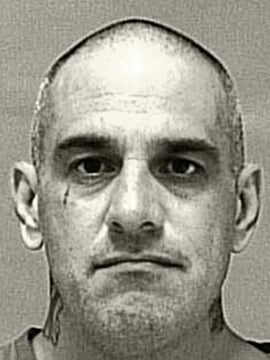
\includegraphics[width=.5\textwidth]{PRATER.jpg}
            \footnotesize
            \begin{itemize}
                \item Prior Offenses: 2 armed robberies, 1 attempted armed robbery
                \item Subsequent Offenses: 1 grand theft
                \item Risk Score: 3
            \end{itemize}
        \end{column}
        \begin{column}{.5\textwidth}
            \centering
            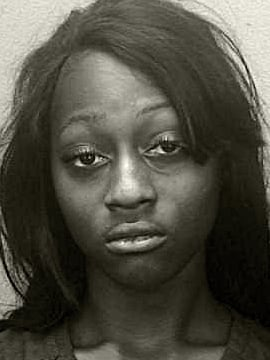
\includegraphics[width=.5\textwidth]{BORDEN.jpg}
            \footnotesize
            \begin{itemize}
                \item Prior Offenses: 4 juvenile misdemeanors
                \item Subsequent Offenses: None
                \item Risk Score: 8
            \end{itemize}
        \end{column}
    \end{columns}
\end{frame}

\begin{frame}
    \frametitle{COMPAS}
    \begin{itemize}
        \item COMPAS is an algorithm
        used by U.S. courts for predicting recidivism based on a
        questionaire.
        \item In 2016, ProPublica found that the algorithm is biased.
        \begin{quote}
            Black defendants were often predicted to be at a higher risk of recidivism than they actually were.
            White defendants were often predicted to be less risky than they were.
        \end{quote}
        \item The false-positive rates vary significantly across
        black people and white people, violating \textit{equalized odds}.
    \end{itemize}
    \footnotetext[1]{\href{https://www.propublica.org/article/how-we-analyzed-the-compas-recidivism-algorithm}{(Link) ProPublica - How We Analyzed the COMPAS Recidivism Algorithm}}
    \footnotetext[2]{\href{https://www.youtube.com/watch?v=TqnYf2h6A-k}{(Link) Vsauce2 - The Dangerous Math Used To Predict Criminals}}
\end{frame}

\begin{frame}
    \frametitle{Fairness Metrics: Equalized Odds}
    \begin{itemize}
        \item Equalized odds measures whether a model's error rates are balanced across groups.
        \item In other words, it asks: \textit{Does the model make mistakes equally, regardless of group membership?}
        \item Formally, it requires that
        \begin{align*}
            \abs{P[\hat{Y} = 1 | S = 1, Y = 0] - P[\hat{Y} = 1 | S \neq 1, Y = 0]} & \leq \epsilon \\
            \abs{P[\hat{Y} = 1 | S = 1, Y = 1] - P[\hat{Y} = 1 | S \neq 1, Y = 1]} & \leq \epsilon
        \end{align*}
        where $\hat{Y}$ is the predicted outcome, $Y$ is the ground truth, and $S$ is the sensitive attribute.
        \item It ensures that both false positive and true positive rates are similar across groups.
    \end{itemize}
\end{frame}

\begin{frame}{Auditing Framework}
    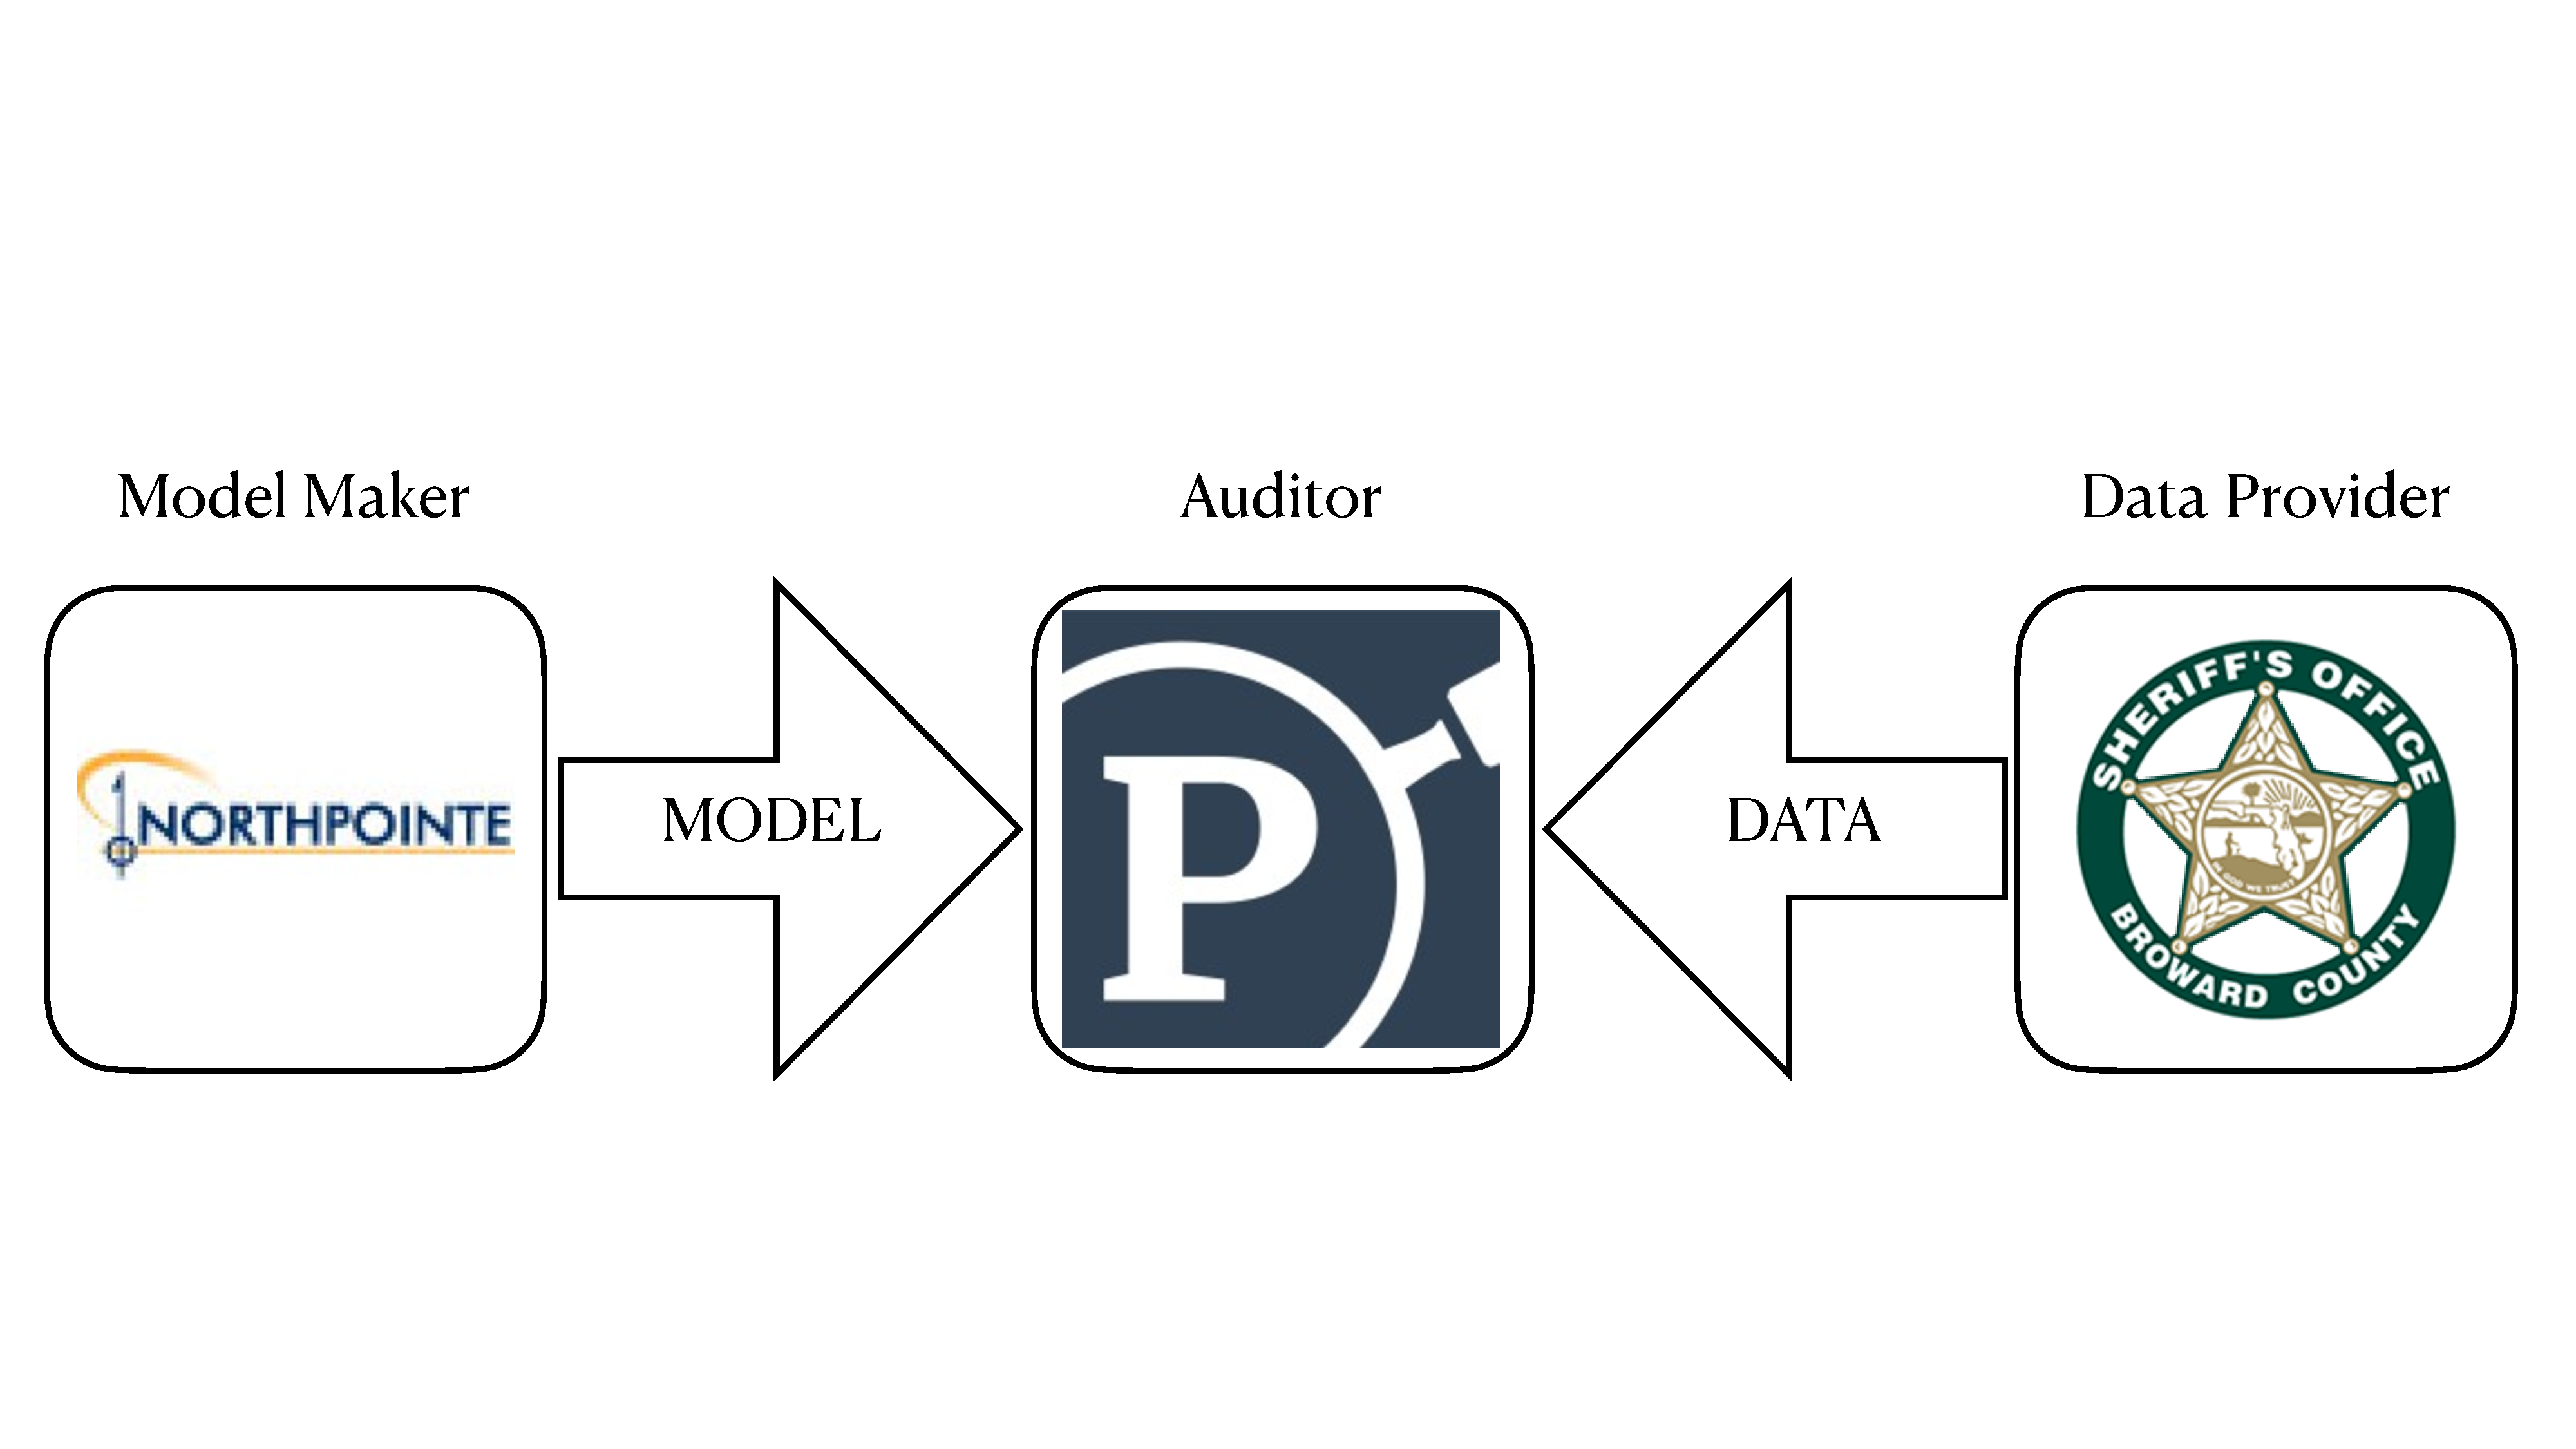
\includegraphics[width=\linewidth]{compas}
\end{frame}

\begin{frame}{The Privacy Problem}
  The COMPAS audit was possible only because the U.S. law made the data
  publicly accessible. Otherwise, such audits would be infeasible.
  \begin{itemize}
    \item Auditors need sensitive data to test fairness.
    \item But holding this data introduces security and privacy risks.
    \item Security risk: hackers could steal the data. \\ Example: \href{https://en.wikipedia.org/wiki/23andMe_data_leak}{(Link) 23andMe data breach}.
    \item Privacy risk: published stats could expose insights. \\ Example: \href{https://pmc.ncbi.nlm.nih.gov/articles/PMC8766950/}{(Link) All of Us inference attack}.
  \end{itemize}
\end{frame}

\begin{frame}{Solution: Privacy-Preserving Audits}
  \begin{itemize}
    \item Use synthetic data generated from real data.
    \item Apply differentially private synthetic data generation techniques to ensure individual info stays hidden.
    \item Auditors only keep the synthetic data and not the real data.
  \end{itemize}
\end{frame}

\begin{frame}{Data Marginals}
  \begin{columns}
    \begin{column}{0.48\textwidth}
      \centering
      \textbf{Original Data}
      \begin{tabular}{|l|l|l|}
        \hline
        \textbf{ID} & \textbf{Sex} & \textbf{Race} \\
        \hline
        1 & Male   & White \\
        2 & Female & White \\
        3 & Female & Black \\
        4 & Male   & Black \\
        5 & Female & Black \\
        6 & Female & White \\
        \hline
      \end{tabular}
    \end{column}

    \begin{column}{0.48\textwidth}
      \centering
      \textbf{(Sex,Race) Marginal}
      \begin{tabular}{|l|l|r|}
        \hline
        \textbf{Sex} & \textbf{Race} & \textbf{Count} \\
        \hline
        Male   & White & 1 \\
        Female & White & 2 \\
        Male   & Black & 1 \\
        Female & Black & 2 \\
        \hline
      \end{tabular}
    \end{column}
  \end{columns}
\end{frame}

\begin{frame}{Differentially Private Synthetic Data}
  \begin{itemize}
    \item Fake data that mimic the real data's patterns.
    \item Generated with differential privacy, which adds noise to marginals to protect privacy.
    \item Lets auditors analyze fairness without exposing personal data.
  \end{itemize}
\end{frame}

\begin{frame}{Noising Marginal}
  \begin{columns}
    \begin{column}{0.48\textwidth}
      \centering
      \textbf{Original Marginal}
      \begin{tabular}{|l|l|r|}
        \hline
        \textbf{Sex} & \textbf{Race} & \textbf{Count} \\
        \hline
        Male   & White & 1 \\
        Female & White & 2 \\
        Male   & Black & 1 \\
        Female & Black & 2 \\
        \hline
      \end{tabular}
    \end{column}

    \begin{column}{0.48\textwidth}
      \centering
      \textbf{Noised Marginal}
      \begin{tabular}{|l|l|r|}
        \hline
        \textbf{Sex} & \textbf{Race} & \textbf{Count} \\
        \hline
        Male   & White & 0.8 \\
        Female & White & 2.1 \\
        Male   & Black & 0.4 \\
        Female & Black & 1.9 \\
        \hline
      \end{tabular}
    \end{column}
  \end{columns}
\end{frame}

\begin{frame}{How The Synthetic Data Are Generated}
  \begin{itemize}
    \item We use a proven method that won a U.S. government competition: \href{https://www.nist.gov/ctl/pscr/open-innovation-prize-challenges/past-prize-challenges/2018-differential-privacy-synthetic}{(Link) NIST 2018}.
    \item It adds noise to protect privacy while preserving overall patterns.
    \item The result: data that looks real but contains no real individuals.
  \end{itemize}
\end{frame}

\begin{frame}{Synthetic Data}
  \begin{columns}

    \begin{column}{0.48\textwidth}
      \centering
      \textbf{Original Data}
      \begin{tabular}{|l|l|l|}
        \hline
        \textbf{ID} & \textbf{Sex} & \textbf{Race} \\
        \hline
        1 & Male   & White \\
        2 & Female & White \\
        3 & Female & Black \\
        4 & Male   & Black \\
        5 & Female & Black \\
        6 & Female & White \\
        \hline
      \end{tabular}
    \end{column}

    \begin{column}{0.48\textwidth}
      \centering
      \textbf{Synthetic Data}
      \begin{tabular}{|l|l|l|}
        \hline
        \textbf{ID} & \textbf{Sex} & \textbf{Race} \\
        \hline
        1 & Male   & White \\
        2 & Female & Black \\
        3 & Female & Black \\
        4 & Male   & White \\
        5 & Female & White \\
        6 & Female & Black \\
        \hline
      \end{tabular}
    \end{column}
  \end{columns}
\end{frame}

\begin{frame}{Does It Work?}
  \begin{itemize}
    \item We experimented on real datsets: Adult, COMPAS, Diabetes.
    \item We compared fairness metrics of original and synthetic data.
    \item Most metrics are within negligible difference.
  \end{itemize}
\end{frame}

\begin{frame}{Equalized Odds on COMPAS: Original vs. Synthetic}
  \centering
  \begin{tabular}{|l|c|c|c|}
    \hline
    \textbf{Metric} & \textbf{Original} & \textbf{Synthetic} & \textbf{Difference} \\
    \hline
    Equalized Odds (False Positive) & 0.0249 & 0.0802 & 0.0553 \\
    Equalized Odds (True Positive)  & 0.0177 & 0.0825 & 0.0648 \\
    \hline
  \end{tabular}
\end{frame}

\begin{frame}{Limitations}
  \begin{itemize}
    \item Results are not guaranteed to be accurate.
    \item Complex patterns may be missed.
    \item Privacy vs precision trade-off.
  \end{itemize}
\end{frame}

\begin{frame}{Policy Implications}
  \begin{itemize}
    \item Enables safer third-party audits under privacy guarantees.
    \item Avoids liability for storing sensitive datasets.
  \end{itemize}
\end{frame}

\begin{frame}{Conclusion}
  \begin{itemize}
    \item Synthetic data can support fairness audits with privacy.
    \item Our framework is practical and provably private.
    \item Opens new pathways for legal oversight of AI systems.
  \end{itemize}

  Slides: \url{https://github.com/RexYuan/Eunectes}.
\end{frame}

\end{document}
